% !TEX root = ../main.tex
\bigskip
\chapter{VIGRA Graph Library} \label{ch:vigra_graph_lib}

VIGRA \cite{software_vigra,koethe_2000_phd_thesis} is a library for image processing and analysis, 
which provides customizable and generic algorithms and data-structures.
The library is capable of dealing with multi-dimensional images 
and many algorithms are implemented for arbitrary data types
and dimensions.
VIGRA has a wide range of features: simple convolution filters, 
tensor based image processing and machine learning algorithms 
as decision trees.

To simplify the implementation of algorithms for images with arbitrary 
dimension, VIGRA uses a grid graph which is capable of
dealing with any dimension.

Within this thesis we extend the concept of graph based image processing
within VIGRA w.r.t. graphs of any structure.
We put main emphasis on extendability while keeping the usage very simple.


%\section{Graph API's}\label{sec:graph_apis}
% !TEX root = ../../main.tex

\section{Graph APIs}\label{sec:graph_apis}



We strongly belief it is beneficial to use an existing graph API,
instead of inventing an own graph API for VIGRA.
Coming up with a new API is not straight forward
since one might to think of any future use case.
In addition, users became accustomed with existing API as 
the LEMON \citep{lemon_lib} or BOOST graph API \citep{ boost_bgl}.
Existing algorithms might be reused, as \cite{straehle_2011_miccai} which is implemented 
within LEMON's API.






\subsection{LEMON Graph API}\label{sec:lemon_graph_apis}
    LEMON \citep{ lemon_lib} 
    stand for  ``Library for Efficient Modeling and Optimization in Networks.''.
    It is an open source C++ library with algorithms and data structures 
    related to directed and undirected graphs.
    The extensive usage of templates makes this library very flexible.
    While LEMON provides a huge set of graph algorithms,
    we are mostly interested in the graph API itself.
    In the following, we will give a brief overview of lemons graph 
    API and the related concepts.
    Explaining the complete  API in detail
    is beyond the scope of this thesis.
    Interested readers are referred to work of \citet{lemon_lib}.
    We will only discuss the API for undirected graphs since any
    graph algorithm we implemented within this thesis
    will work on undirected graphs exclusively.

\paragraph{Graph Items :}
    Any undirected graph class fulfilling the LEMON API needs to define 
    the following \emph{descriptor} types to represent the graph items:
    \begin{inparaenum}[(i)]
    \item \lstinline{Graph::Node},
    \item \lstinline{Graph::Edge} and
    \item \lstinline{Graph::Arc}.
    \end{inparaenum}
    These \emph{descriptor} should be cheap types which can be copied
    and passed with almost no overhead.
    In addition, each descriptor has an unique id
    \footnote{ unique id w.r.t. the item type. 
    Therefore  multiple  nodes cannot have the same id.
    The same holds line for edges and arcs.
    But there might be a node and edge which have the same id}.
    These ids can be accessed via \lstinline{Graph::id(Node)}, \lstinline{Graph::id(Edge)} and \lstinline{Graph::id(Arc)}.
    These ids can not only be dense but also sparse, which is very
    important for an efficient handling of grid graph edge ids (see \cref{sec:graphs_grid_graph}).


\phantomsection
\label{par:lemon_iterators}
\paragraph{Iterators :}
    Within LEMON a very convenient mechanism is used to iterate over
    nodes, edges and arcs.
    A special constant \lstinline{INVALID} is used to determine if 
    an iterator reached the end.

    \begin{lstlisting}[language=c++]
    // iterate over nodes
    for(Graph::NodeIt v(g); v!= lemon::INVALID; ++v){/*...*/}

    // iterate over edges
    for(Graph::EdgeIt e(g); e!= lemon::INVALID; ++e){/*...*/}

    // iterate over arcs
    for(Graph::ArcIt a(g); a!= lemon::INVALID; ++a){/*...*/}

    // use arcs to iterate over neighbor nodes
    for(Graph::OutArcIt a(g,n); a!= lemon::INVALID; ++a){
        const Node neighborNode = g.target(a);
        /*...*/
    }
    \end{lstlisting}

    Any iterator is convertible to the corresponding item which
    is iterated without using \lstinline{operator*()}.

\paragraph{Map Concept :}
    The separation between the graph, and data which is related to
    the graph is crucial.
    Different algorithms which operate on the same graph will
    need different data attached to the edges, nodes and arcs. 

    In LEMON, graph classes store only the structure of the graph itself.
    All addition data for nodes, edges and arcs is stored 
    in \emph{maps}.
    The API for graph maps in lemon is very small and easy to implement.
    In fact, only a constructor and \lstinline{operator[](...)} needs
    to be implemented (see \cref{fig:uml_lemon_graph_concepts} for an UML class diagram).



    \begin{figure}[H]
    \begin{center}
        \begin{tikzpicture}[scale=0.55,transform shape]
            \begin{umlpackage}{LEMON API}
                    \umlclass[x=-15.5,y=0]{UndirectedGraphConcept}
                {
                }
                {
                    // Typedefs \usp \\
                    + Node \usp \\
                    + Edge \usp \\
                    + Arc  \usp \\
                    + NodeIt \usp \\
                    + EdgeIt \usp \\
                    + ArcIt  \usp \\
                    + IncEdgeIt \usp \\
                    + InArcIt   \usp \\
                    + OutArcIt  \\

                    // Nested Classes  \\
                    + NodeMap \nestedtemp{ValueType}   \\
                    +  EdgeMap \nestedtemp{ValueType}   \\
                    +  ArcMap \nestedtemp{ValueType}   \\

                    // Member Functions
                    + u(edge : Edge) : Node \usp \\
                    + v(edge : Edge) : Node \usp \\
                    + source(arc : Arc) : Node \usp \\
                    + target(arc : Arc) : Node \usp \\
                    + id(node : Node) : int \usp \\
                    + id(edge : Edge) : int \usp \\
                    + id(arc  : Arc)  : int \usp \\
                    + nodeFromId(id : int) : Node \usp \\
                    + edgeFromId(id : int) : Edge \usp \\
                    + arcFromId(id  : int) : Arc  \usp \\
                    + maxNodeId() : int \usp \\
                    + maxEdgeId() : int \usp \\
                    + maxArcId()  : int \usp \\
                    + direction(arc : Arc) : bool \usp \\
                    + direct(edge : Edge, naturalDirection : bool) :Arc \usp \\
                    + direct(edge : Edge, node : Node) :Arc \usp \\
                    + oppositeArc(arc : Arc) : Node \usp \\
                    + oppositeNode(node : Node, edge : Edge) : Node \usp \\
                    + baseNode(iter : IncEdgeIt) : Node \usp \\
                    + runningNode(iter : IncEdgeIt) : Node \usp \\
                    + baseNode(iter : OutArcIt) : Node \usp \\
                    + runningNode(iter : OutArcIt) : Node \usp \\
                    + baseNode(iter : InArcIt) : Node \usp \\
                    + runningNode(iter : InArcIt) : Node 
                }
                %\begin{umlpackage}{Graph Item Concept}
                    \umlclass[x=-6.5,y=7]{Node}
                    {
                    }
                    {   
                        + Node() \usp \\ 
                        + Node(node : Node) \usp \\ 
                        + Node(invalid: Invalid)  \usp \\ 
                        + operator == (node : Node) : bool \usp \\ 
                        + operator != (node : Node) : bool \usp \\ 
                        + operator <  (node : Node) : bool \usp \\ 
                        \quad
                    } 
                    \umlclass[x=0,y=7]{Edge}
                    {
                    }
                    {  
                        + Edge() \usp \\ 
                        + Edge(edge : Edge) \usp \\ 
                        + Edge(invalid: Invalid)  \usp \\ 
                        + operator == (edge : Edge) : bool \usp \\ 
                        + operator != (edge : Edge) : bool \usp \\ 
                        + operator <  (edge : Edge) : bool \usp \\
                        \quad
                    } 
                    \umlclass[x=6.5,y=7]{Arc}
                    {
                    }
                    {   
                        + Arc() \usp \\ 
                        + Arc(arc : Arc) \usp \\ 
                        + Arc(invalid: Invalid)  \usp \\ 
                        + operator == (arc : Arc) : bool \usp \\ 
                        + operator != (arc : Arc) : bool \usp \\ 
                        + operator <  (arc : Arc) : bool \usp \\ 
                        + operator Edge () : Edge 
                    } 
                %\end{umlpackage}


                %\begin{umlpackage}{Graph Item Iterator Concept}
                    \umlclass[x=-7,y=0]{NodeIt}
                    {
                    }
                    {   
                        + NodeIt() \usp \\ 
                        + NodeIt(iter : NodeIt) \usp \\ 
                        + NodeIt(invalid: Invalid)  \usp \\ 
                        + NodeIt(g: Graph)  \usp \\ 
                        + NodeIt(g: Graph, node: Node)  \usp \\ 
                        + operator++(): NodeIt \\ 
                    }
                    \umlclass[x=0,y=0]{EdgeIt}
                    {
                    }
                    {   
                        + EdgeIt() \usp \\ 
                        + EdgeIt(iter : EdgeIt) \usp \\ 
                        + EdgeIt(invalid: Invalid)  \usp \\ 
                        + EdgeIt(g: Graph)  \usp \\ 
                        + EdgeIt(g: Graph, edge: Edge)  \usp \\ 
                        + operator++(): EdgeIt \\ 
                    }
                    \umlclass[x=7,y=0]{ArcIt}
                    {
                    }
                    {   
                        + ArcIt() \usp \\ 
                        + ArcIt(iter : ArcIt) \usp \\ 
                        + ArcIt(invalid: Invalid)  \usp \\ 
                        + ArcIt(g: Graph)  \usp \\ 
                        + ArcIt(g: Graph, arc: Arc)  \usp \\ 
                        + operator++(): ArcIt \\ 
                    } 
                %\end{umlpackage}


                %\begin{umlpackage}{Graph Neighborhood Iterator Concept}
                    \umlclass[x=-7.5,y=-7]{IncEdgeIt}
                    {
                    }
                    {   
                        + IncEdgeIt() \usp \\ 
                        + IncEdgeIt(iter : IncEdgeIt) \usp \\ 
                        + IncEdgeIt(invalid: Invalid)  \usp \\ 
                        + IncEdgeIt(g: Graph, node: Node)  \usp \\ 
                        + IncEdgeIt(g: Graph, node: Node, edge : Edge)  \usp \\ 
                        + operator++(): IncEdgeIt \\ 
                    }
                    \umlclass[x=0,y=-7]{InArcIt}
                    {
                    }
                    {   
                        + InArcIt() \usp \\ 
                        + InArcIt(iter : InArcIt) \usp \\ 
                        + InArcIt(invalid: Invalid)  \usp \\ 
                        + InArcIt(g: Graph, node: Node)  \usp \\ 
                        + InArcIt(g: Graph, node: Node, arc : Arc)  \usp \\ 
                        + operator++(): InArcIt \\ 
                    }
                    \umlclass[x=7.5,y=-7]{OutArcIt}
                    {
                    }
                    {   
                        + OutArcIt() \usp \\ 
                        + OutArcIt(iter : OutArcIt) \usp \\ 
                        + OutArcIt(invalid: Invalid)  \usp \\ 
                        + OutArcIt(g: Graph, node: Node)  \usp \\ 
                        + OutArcIt(g: Graph, node: Node, arc : Arc)  \usp \\ 
                        + operator++(): OutArcIt \\ 
                    }
                    \umlclass[x=-13,y=-16]{NodeMap}
                    {
                    }
                    {   
                        // Typedefs \\
                        + Value \\
                        + ConstReference \\
                        + Reference \\
                        + Key // same as Node for NodeMap \\
                        \\// Members \\
                        +NodeMap(graph : Graph ) \\
                        + operator[](edge : Key) : Reference \\
                        + operator[](edge : Key) : ConstReference \\
                    } 
                    \umlclass[x=-6,y=-16]{EdgeMap}
                    {
                    }
                    {   
                        // Typedefs \\
                        + Value \\
                        + ConstReference \\
                        + Reference \\
                        + Key // same as Edge for EdgeMap \\
                        \\// Members \\
                        +EdgeMap(graph : Graph ) \\
                        + operator[](edge : Key) : Reference \\
                        + operator[](edge : Key) : ConstReference \\
                    } 
                    \umlclass[x=1,y=-16]{ArcMap}
                    {
                    }
                    {   
                        // Typedefs \\
                        + Value \\
                        + ConstReference \\
                        + Reference \\
                        + Key // same as Arc for ArcMap \\
                        \\// Members \\
                        +ArcMap(graph : Graph ) \\
                        + operator[](arc : Key) : Reference \\
                        + operator[](arc : Key) : ConstReference \\
                    } 

                %\end{umlpackage}


                \umlinherit[]{NodeIt}{Node}
                \umlinherit[]{EdgeIt}{Edge}
                \umlinherit[]{ArcIt}{Arc}

                \umlinherit[]{IncEdgeIt}{Edge}
                \umlinherit[]{InArcIt}{Arc}
                \umlinherit[]{OutArcIt}{Arc}

            \end{umlpackage}
        \end{tikzpicture}
    \end{center}
    \caption{
        UML class diagram of most important LEMON concepts.
        UndirectedGraphConcept shows LEMON's API for undirected 
        graphs. Any graph implemented within LEMON's API 
        needs to implement all methods and typedefs showed 
        in the UML diagram.
        To implement a graph class within the API one needs 
        to implement descriptor classes for nodes, edges and arcs.
        These descriptor classes have almost no API.
        The graph itself is responsible to deal with them.
        The descriptors are usually implemented as cheap classes,
        and are used to \emph{describe} a node, and do not implement
        functionality for nodes.
        The functionality comes from the graph class itself.
        Iterators in LEMON are somehow different from usual 
        iterators, instead of an end iterator, lemon used a special
        class \lstinline{lemon::INVALID}, and all iterators
        need to comparable with \lstinline{lemon::INVALID} (see \cref{par:lemon_iterators}).
    }\label{fig:uml_lemon_graph_concepts}
    \end{figure}






    %\begin{minipage}{\textwidth}
        Any graph has a templated default implementations for graph maps.
        An edge map with \lstinline{float} as value type, which might
        be used as an edge indicator/weight, can be 
        used in the following way.

        \begin{lstlisting}[language=c++]
        // edge map (for data as edge weights)
        Graph::EdgeMap<float> edgeMap(g); 
        for(Graph::EdgeIt e(g); e!= lemon::INVALID; ++e){
            const float val = edgeMap[*e];  // read
            edgeMap[*e] = std::exp(-1.0*a); // write
        }
        \end{lstlisting}
    %\end{minipage}

    %\begin{minipage}{\textwidth}
        A node map with  \lstinline{unsigned int} as value type,
        which could encode a labeling for a graph 
        can be accessed as shown below.

        \begin{lstlisting}[language=c++]
        // node map (for node related data as node labelings )
        Graph::NodeMap<usigned int> nodeMap(g);
        for(Graph::NodeIt v(g); v!= lemon::INVALID; ++v){
            const unsigned int val = nodeMap[*v]; // read
            nodeMap[*v] = val+1;                  // write
        }
        \end{lstlisting}
    %\end{minipage}


    % %\begin{minipage}{\textwidth}
    %     Implicit read only graph maps can be implemented very easy and 

    %     \begin{minipage}{\textwidth}\vspace{-0.75cm}\begin{lstlisting}[language=c++]
    %     template<class Graph>
    %     class ImplicitEdgeMap {
    %     public:
    %         typedef typename Graph::Edge Key;
    %         typedef double Value;
    %         ImplicitEdgeMap(const Graph & graph){
    %             /*
    %                 constructor code here
    %             */
    %         }
    %         Value operator[](const Key & edge) const { 
    %             Value a;
    %             /*
    %                 compute a value for the edge
    %                 implicity here
    %             */
    %             return a;
    %         }
    %     };
    %     \end{lstlisting}\end{minipage}\vspace{0.5cm}
    % %\end{minipage}

\subsection{BOOST Graph API}\label{sec:boost_graph_apis}
The BOOST Graph Library (BGL)  \citep{boost_bgl} is set of data structures and 
algorithms for graph related computations.
Since all  data-structures and algorithms presented within this thesis  are implemented within the LEMON graph interface, 
the BGL graph API will only be described briefly.

The main difference between the LEMON graph API and the BGL,
is the massive usage of trait classes and free functions within the BGL.
While LEMON classes use typedefs and member functions, 
the BGL uses trait classes and free functions which need 
to be implemented or specialized for a particular graph.

Node and edge descriptors are used in the same way as in LEMON's
graph API \footnote{within BGL these descriptors are called \lstinline{vertex_descriptor} and 
\lstinline{node_descriptor}}.
There are no restrictions how these descriptors can be implemented.
For most graph algorithms, the BGL expects a list of dense integers for
node and edge ids.
With this requirement, any flexibility of custom edge and node descriptors is lost.
We belief that this is a poor design choice, since sparse ids
are crucial for most graphs (see \cref{sec:impl_graphs}).




\subsection{VIGRA Graph API}

While the grid graph is implemented within the BGL and LEMON graph API,
all algorithms and data-structures implemented within this thesis will
use the LEMON graph API instead of the BGL 
for the following reasons:
\begin{inparaenum}[(i)]
\item Algorithms using the BGL API expect not only the graph, but also 
a list of dense integers, while LEMON allows for sparse ids which 
are part of the graph itself.
\item LEMON seems to be well maintained and under active development,
while for the BGL there is no current development at all.
\item The documentation of LEMON is excellent, while the BGL is
documented in a very confusing way.
  
\end{inparaenum}

 

%\section{Implementation}\label{sec:vigra_graph_lib_impl}
% !TEX root = ../../main.tex


\section{Implementation}\label{sec:vigra_graph_lib_impl}

\todo{Impl is not a good word here}

The most important concept for graph based image processing
is the \emph{region adjacency graph} (RAG) (see \cref{fig:make_rag}).

A RAG is extracted from a labeled \emph{base graph}.
In the first step of graph based image processing, the base 
graph is usually a grid graph, and the labeling is a label image
as in \cref{fig:make_rag} .
To encode a RAG we need a undirected graph, 
and a mapping from the base graphs edges and nodes to the RAG 
needs to be stored.

The implementation of grid graphs is explained in \cref{sec:graphs_grid_graph}, 
a basic undirected graphs implementation will be discussed in \cref{sec:graphs_adjacency_list_graph}.
The implementation details of the \emph{region adjacency graph} concept will 
be given in  \cref{sec:graphs_rag}.

For hierarchical clustering we provide a specialized graph, named \emph{merge graph}.


To implemented structured clustering algorithms (see \cref{sec:rw_hc}) we
need a graph which supports the contraction of edges.
Also a mechanism to merge node and edge features is needed.
Within \cref{sec:graphs_merge_graph} we propose  a very flexible graph 
called \emph{merge graph adaptor} which fulfills these requirements.


A generic set of algorithms which work on any graph
implemented within the VIGRA graph api is presented 
in \cref{sec:graph_graph_algorithms}.

While the core implementation of any algorithm is in C++
VIGRA provides python binding to make almost
any algorithm available in Python.
To provide a generic Python interface for any proposed
graph, we need to introduce a few concepts 
to make the python wrapped graph API very \emph{Pythonic}


%$\surd \bullet$


\begin{table}
\begin{tiny}
\begin{tabular}{|l|p{1.5cm}|p{0.5cm}|p{0.5cm}|p{0.6cm}|p{0.6cm}|p{0.6cm}|p{0.8cm}|p{0.8cm}|l|l|l|}
    \hline 
    Class & purpose & 
        add nodes & add edges & contract edges & node ids & edge ids & 
        node descriptor & edge descriptors &
        node map & edge map  &
        header
    \\ \hline
    %
    2D-GridGraph & implicit graph for 2D images & 
        x & x & x & dense & sparse & 
        $\colvec{x\\y}$ &  $\colvec{x\\y\\e}$ & 
        2D-Array & 3D-Array   &
        \detokenize{multi_gridgraph.hxx}
    \\ \hline
    %
    3D-GridGraph & implicit graph for 3D volumes & 
        x & x & x & dense & sparse & 
        $\colvec{x\\y\\z}$ &  $\colvec{x\\y\\z\\e}$ & 
        3D-Array & 4D-Array   &
        \tiny{\detokenize{multi_gridgraph.hxx}}
    \\ \hline
    %
    4D-GridGraph & implicit graph for 3D volumes $+$ time & 
        x & x & x & dense & sparse & 
        $\colvec{x\\y\\z\\t}$ &  $\colvec{x\\y\\z\\t\\e}$ & 
        4D-Array & 5D-Array   &
        \detokenize{multi_gridgraph.hxx}
    \\ \hline
    %
    AdjacencyListGraph & multi purpose graph & 
       $\bullet$  & $\bullet$ & x & maybe dense & dense & 
       $\colvec{n}$ , same as node id &  $\colvec{e}$  , same as edge id & 
       1D-Array & 1D-Array   &
       \detokenize{adjacency_list_graph.hxx}
    \\ \hline
    %
    MergeGraphAdpator & edge contraction with feature merging callback & 
       x & x & $\bullet$& sparse & sparse & 
       $\colvec{n}$ , same as node id &  $\colvec{e}$ , same as edge id & 
       1D-Array & 1D-Array   &
       \detokenize{merge_graph_adaptor.hxx}
    \\ \hline
\end{tabular}
\end{tiny}
\end{table}
\subsection{Graphs}

\subsubsection{Grid Graph} \label{sec:graphs_grid_graph}

The grid graph implemented in VIGRA is N-dimensional.
The dimension can be selected with templates, and therefore with zero
overhead.

Due to the regular structure of a grid graph, it is possible to compute the edges of a given 
node and vice versa on the fly, instead of storing these relations explicitly.
Therefore a grid graph can be implemented with almost zero memory overhead.

\paragraph{Node Descriptor/Id :}
The node descriptor of a grid graph is implemented as a
$N$-dimensional coordinate of the pixel which corresponds to
that particular node. The id of a node is the scan order index
of the corresponding pixel.
As a consequence, node id's of a grid graph are continuous.
\paragraph{Edge Descriptor/Id :}
To edge descriptors are implemented as $N+1$-dimensional coordinate.
The first $N$ axis correspond to the node which ``owns'' this edge.
The last axis enumerates the edge w.r.t. the node.

In a grid graph, all nodes have the same degree, except for nodes
at the border of the image.
This breaks somehow the regularity of grid graphs.
To still have very regular structure, edge ids
are enumerated, as if the graph would be perfectly
regular. Therefore we enumerate some missing edges
at the border and get non-continuous edge ids.
\Cref{fig:grid_graph_ids} illustrates this enumeration.



\begin{figure}[H]
\centering
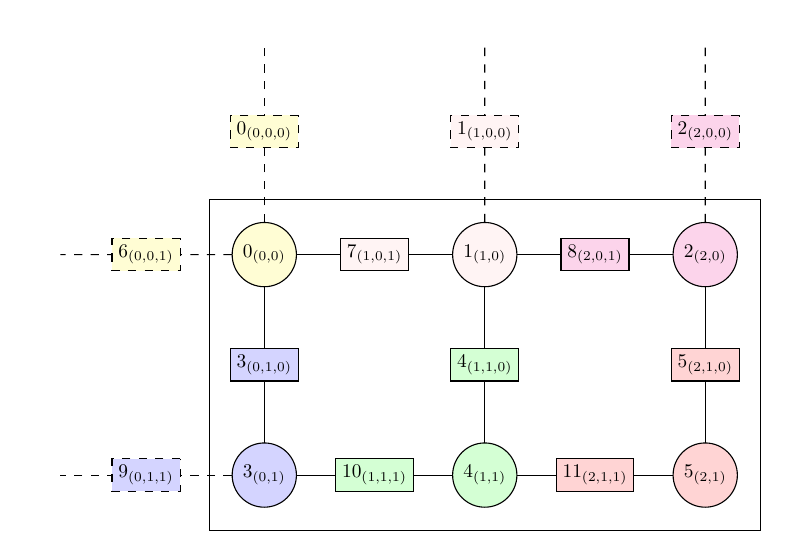
\begin{tikzpicture}[scale=0.7,transform shape]
  % virtual nodes
  \draw (-2*2,0) node (naa) {$\quad$};
  \draw (-2*2,2*2) node (nbb) {$\quad$};
  \draw (0,4*2) node (na) {$\quad$};
  \draw (2*2,4*2) node (nb) {$\quad$};
  \draw (4*2,4*2) node (nc) {$\quad$};
  % real nodes
  \draw (0,0) node[draw,circle,fill=blue!17] (n3) {$3_{(0,1)}$};
  \draw (2*2,0) node[draw,circle,fill=green!17] (n4) {$4_{(1,1)}$};
  \draw (4*2,0) node[draw,circle,fill=red!17] (n5) {$5_{(2,1)}$};
  \draw (0,2*2) node[draw,circle,fill=yellow!17] (n0) {$0_{(0,0)}$};
  \draw (2*2,2*2) node[draw,circle,fill=pink!17] (n1) {$1_{(1,0)}$};
  \draw (4*2,2*2) node[draw,circle,fill=magenta!17] (n2) {$2_{(2,0)}$};
  %
  % real edges
  \path[every node/.style={auto=false}]
    (n0) edge node[draw,rectangle,fill=pink!17] {$7_{(1,0,1)}$} (n1) 
    (n1) edge node[draw,rectangle,fill=magenta!17] {$8_{(2,0,1)}$} (n2) 
    (n3) edge node[draw,rectangle,fill=green!17] {$10_{(1,1,1)}$} (n4) 
    (n4) edge node[draw,rectangle,fill=red!17] {$11_{(2,1,1)}$} (n5);
 \path[every node/.style={auto=false}]
    (n0) edge node[draw,rectangle,fill=blue!17] {$3_{(0,1,0)}$} (n3) 
    (n1) edge node[draw,rectangle,fill=green!17] {$4_{(1,1,0)}$} (n4) 
    (n2) edge node[draw,rectangle,fill=red!17] {$5_{(2,1,0)}$} (n5) ;
  %
  %virtual edges x
  \path[every node/.style={auto=false}]
    (n0) edge[dashed] node[draw,rectangle,fill=yellow!17] {$0_{(0,0,0)}$} (na) 
    (n1) edge[dashed] node[draw,rectangle,fill=pink!17] {$1_{(1,0,0)}$} (nb) 
    (n2) edge[dashed] node[draw,rectangle,fill=magenta!17] {$2_{(2,0,0)}$} (nc) ;
  \path[every node/.style={auto=false}]
    (n0) edge[dashed] node[draw,rectangle,fill=yellow!17] {$6_{(0,0,1)}$} (nbb) 
    (n3) edge[dashed] node[draw,rectangle,fill=blue!17] {$9_{(0,1,1)}$} (naa) ;
   %
   \draw (-1.0,5.0) --  (9,5.0) -- (9,-1.0) -- (-1.0,-1.0) -- cycle;
\end{tikzpicture}
\caption[Grid Graph Ids]{ \label{fig:grid_graph_ids}
    Ids and descriptors for a 2D Grid graph with 4-neighborhood on a $3x2$ grid.
    The node ids are continuous from $0$ to $5$ and the descriptors
    are showed as subscripts of the ids.
    Node descriptors are 2D pixel coordinates.
    To get the edge ids, we enumerate the edge, but we ignore the fact that nodes at the
    left and upper border do
    not have an upper and left edge.
    To illustrate this, these ``virtual'' edges are shown dotted.
    The id's of the edges correspond to the enumeration.
    As a consequence edge ids are non continuous.    
    In this examples, 
    the set of valid edge ids is $\{ 3,4,5,7,8,10,11 \}$.
    Edge descriptors are 3D coordinates, where the first two
    coordinate correspond to the node which owns this edge.
    The third coordinate is the edge number w.r.t. the node.
    The two edges and the node which ``owns'' them are
    shown in the same unique color.

}
\end{figure}

\paragraph{Node Map :} An regular N-dimensional image can
be used as node map, and since node descriptors are plain
coordinates, they can be used to access data at a
particular pixel.
This means, no node map needs to be allocated for a given
image, since the image itself can be used as a node map.
The default node map is derived from \lstinline{vigra::MultiArray<DIM,T>}.

\paragraph{Edge Map :} An N+1-dimensional image is
used as edge map.
This image has the same as a node map, but an extra
dimension for the edges.
The first $N$ axis in the edge descriptor are 
used to determine which pixel ``owns'' the edge,
while the last axis select the w.r.t. the node.
The default edge map is derived from \lstinline{vigra::MultiArray<DIM,Multiband<T> >}.

\paragraph{Usage :}
    ...write me
\subsubsection{Adjacency List Graph} \label{sec:graphs_adjacency_list_graph}

\paragraph{Node Descriptor/Id :}
The node descriptor is implemented as a simple class
holding a single integer which is the id 
of the node.
The user can explicitly choose the id of
an node. As a consequence, node id's can 
be sparse and continuous.

\paragraph{Edge Descriptor/Id :}
The edge descriptors are implemented exactly like
node descriptors, but users cannot give
edges explicit id's.
Therefore edge id's are dense, unless
edges are removed from the graph \footnote{Removing edges from the graph is
not yet implemented}.

\paragraph{Node Map, EdgeMap:} 
The node and edge maps are derived from \lstinline{vigra::MultiArray<1,T>}.
Their size is to \lstinline{maxNodeId()+1} and  \lstinline{maxEdgeId()+1}.
The id and the descriptors can be used to index node and edge maps.


\paragraph{Usage :}
    \begin{lstlisting}[language=c++]
    typedef vigra::AdjacencyListGraph Graph;
    Graph g;

    // add nodes 
    // - automatic id
    // - explicit id
    Graph::Node n0 = g.addNode() 
    Graph::Node n3 = g.addNode(3)

    // add edges from existing nodes
    // and new nodes
    // no parallel edges 
    Graph::Edge e0 = g.addEdge(n0,n1)
    Graph::Edge e1 = g.addEdge(2,3)
    Graph::Edge e2 = g.addEdge(2,3)
    assert(e1==e2)  
    \end{lstlisting}

    \begin{lstlisting}[language=Python]
    g=vigra.graphs.listGraph();
    # add nodes 
    # - automatic id
    # - explicit id
    n0 = g.addNode() 
    n3 = g.addNode(3)

    # add edges from existing nodes
    # and new nodes
    # no parallel edges 
    e0 = g.addEdge(n0,n1)
    e1 = g.addEdge(2,3)
    e2 = g.addEdge(2,3)
    assert e1==e2  
    \end{lstlisting}
\subsubsection{Region Adjacency Graph} \label{sec:graphs_rag}

A region adjacency is always defined w.r.t. a labeled base graph.
Instead of implementing a new graph for RAG, we use
the \emph{adjacency list graph}.
The mapping from base graph nodes and RAG nodes  is defined
by the labeling itself. Therefore
The labeling defines a forward mapping from base graph nodes
to RAG Node ids.
Edges in the RAG are mapped to multiple edges in the base graph
via a backward mapping.




\subsubsection{Merge Graph} \label{sec:graphs_merge_graph}

To implemented structured clustering algorithms (see \cref{sec:rw_hc} ) 
A graph which supports edge contraction and feature merging is needed.
Some graphs within the LEMON library support 
edge contraction, but this is not part of LEMON undirected graph concept \footnote{
Edge contraction cannot be a part of LEMON undirected graph concept,since some graphs
are not mutable.}.

\begin{figure}[H]
    \centering
    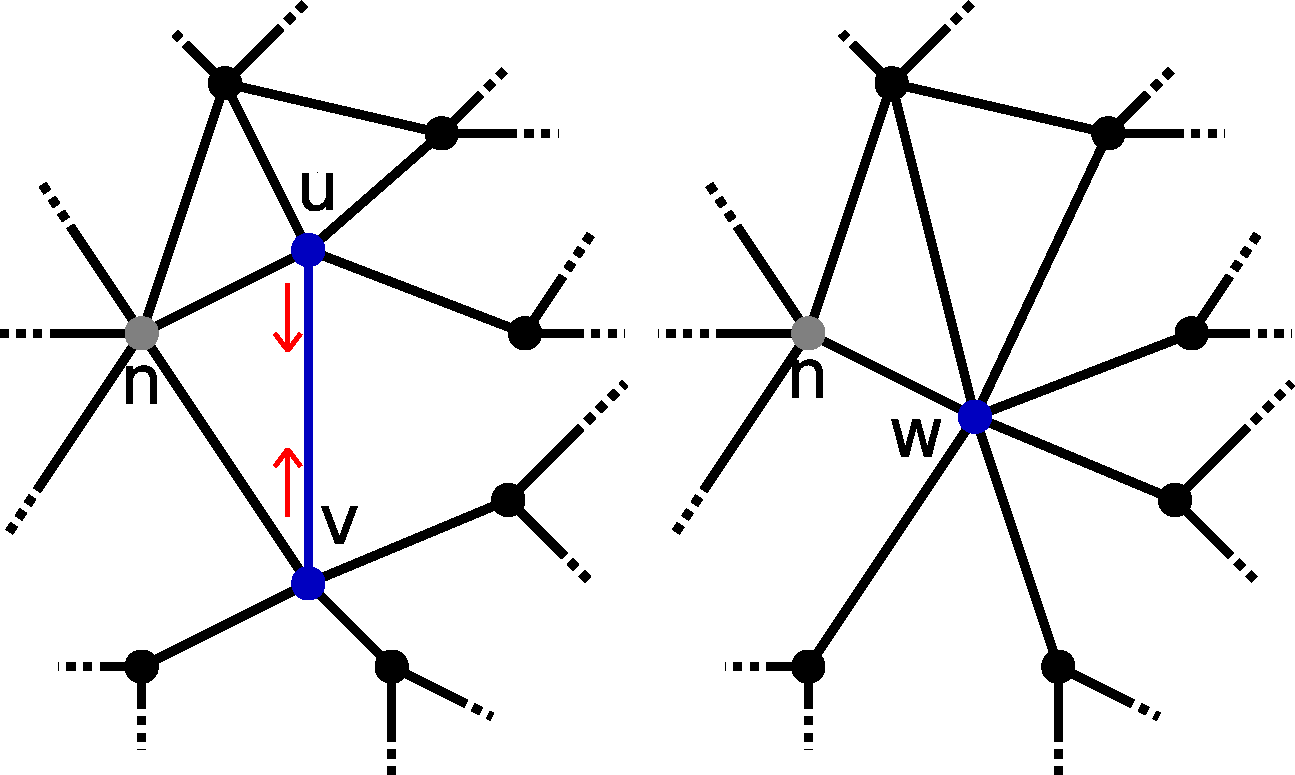
\includegraphics[width=0.35\textwidth]{fig/contraction.pdf}

    \addtocontents{lof}{%
        \vspace{1cm}
        \protect\centerline{%
            \protect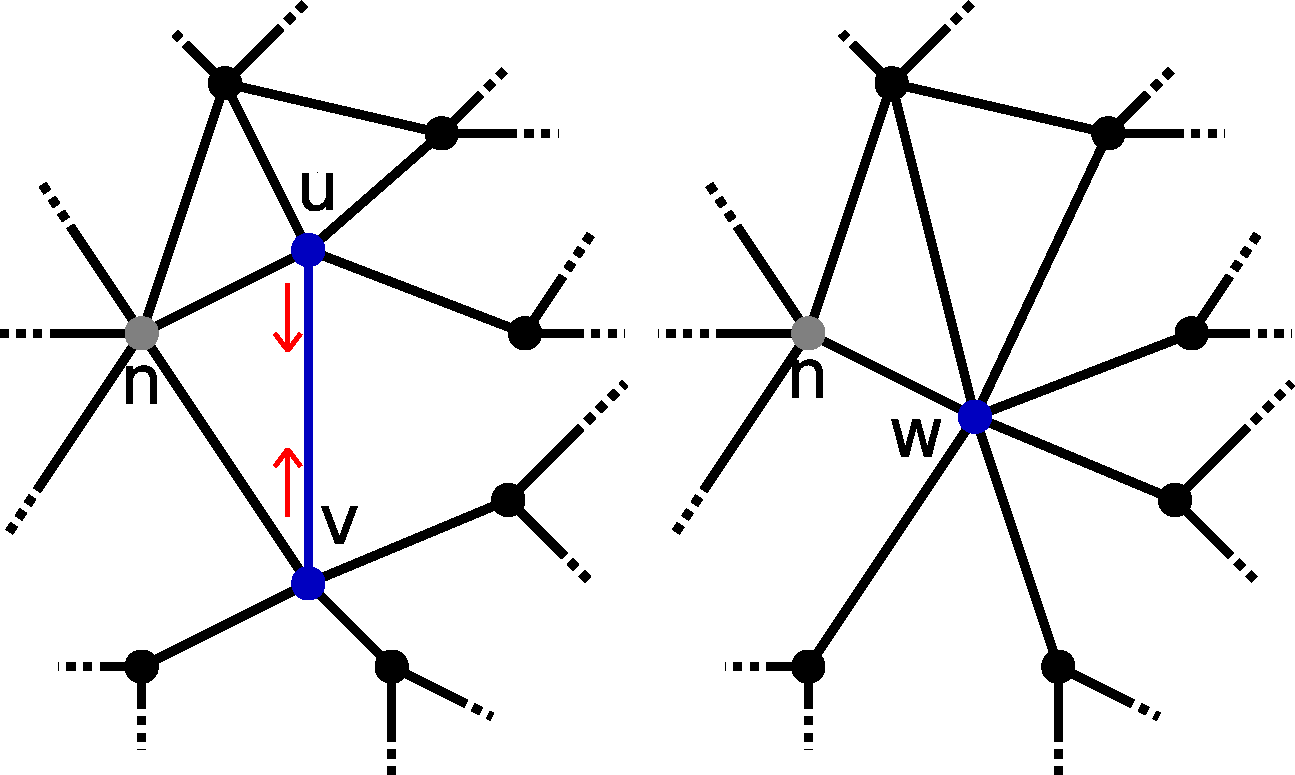
\includegraphics[width=\lofthumbsize,height=\lofthumbsize,keepaspectratio=true]{fig/contraction.pdf} 
        } 

    }%
    \caption[Schematic edge contraction]{ Schematic edge contraction: Node $u$ and $v$ is merged into node $w$.
        Note the gray node $n$ which is connected to $u$ and $v$.
        After the contraction, edges $\{ n,u\}$ and $\{ n,v\}$ are also merged into 
        a single edge $\{ n, w\}$.
        The picture has been taken from \citep{wiki_edge_contraction} and has been modified slightly.
    }
    \label{fig:figlabel}
\end{figure}


Furthermore LEMON does not define any concept for feature merging, which
is crucial for image processing application \citep{arbelaez_2006_cvpr}.
As a consequence, we define a new concept / API for 
edge contraction and feature merging within the philosophy of LEMON.

We implemented the \emph{merge graph} as an LEMON  \href{http://lemon.cs.elte.hu/pub/doc/latest/a00592.html}{graph adaptor}
\footnote{ LEMON Graph Adaptor: \url{http://lemon.cs.elte.hu/pub/doc/latest/a00592.html} }.
A graph adaptor is aways a viewing to a base graph and cannot exist without one.
A subgraph adaptor can used to get view to a subgraph w.r.t. the base graph, without
the need to reallocate the complete subgraph.
In a similar manner, we implement a \emph{merge graph adaptor}.

Each node and edge in the merge graph adaptor corresponds to a connected component of 
edge and nodes in the base graph.
Two union find data structure (UFD), and edge and node ufd encode these connected components.

Feature merging is done via \emph{callbacks} which can be registered to the merge graph adaptor.
The \emph{callback API} is explained in detail below. 


\begin{figure}[H]
\begin{center}
    \begin{tikzpicture}[scale=0.65,transform shape]
        \umlclass[template=Graph]{MergeGraphAdpator}
        {
            - edgeUfd               : IterablePartiton          \\
            - nodeUfd               : IterablePartiton          \\ 
            - nodesAdjacency        : AdjacencySetVector        \\
            - baseGraph             : Graph                     \\
            - mergeNodeCallBacks    : MergeNodeCallBackVector   \\
            - mergeEdgeCallBacks    : MergeEdgeCallBackVector   \\
            - eraseEdgeCallBacks    : EraseEdgeCallBackVector   
        }
        {
            // LEMON API for undirected graphs                  \\
                $\ldots$                                        \\
            // register callbacks                               \\ 
            + registerMergeNodeCallBack(f : MergeNodeCallBack)  \\
            + registerMergeEdgeCallBack(f : MergeEdgeCallBack)  \\
            + registerEraseEdgeCallBack(f : EraseEdgeCallBack)  \\
            // modify graph                                     \\
            + contractEdge(edge : Edge)     : Node              \\
            // find representatives                             \\
            + reprNode(node : Graph::Node)  : Node              \\
            + reprEdge(edge : Graph::Node)  : Edge              \\ 
            // get base graph                                   \\
            + graph()                       : Graph             \\
        } 
    \end{tikzpicture}
\end{center}\caption[Merge Graph Adaptor Class Diagram]{ \label{fig:cls_mga}
    Merge Graph Adaptor Class Diagram.
    Only member functions which are not part of the LEMON
    undirected graph concept are listed. 
    See \cref{fig:uml_lemon_graph_concepts} for all missing 
    members.
}
\end{figure}



\paragraph{Node Descriptor/Id :}
The node descriptor is implemented as a simple class
holding a single integer which is the id 
of the node.
Each node in the merge graph encodes a connected
component of nodes in the base graph.
If no edge has been contracted, the node ids
of the merge graph are identical with the ids 
of the base graph.
The contraction of a single edge will invalidate
one node id, since two nodes are merged into a single 
node.
The connected component membership of base graph
nodes is stored in a union find data structure 
and can be accessed via \lstinline{MergeGraph::reprNode(const BaseGraphNode & baseGraphNode)}.


\paragraph{Edge Descriptor/Id :}
Edge descriptors are implemented as node descriptors.
The contraction of a single edge will invalidate
at least one edge id, since the contracted edge is removed
from the graph.
But contracting a single edge can lead to an
unbounded number of parallel edges / multi edges.
Multiple edges between a pair of nodes will be merged
into single edges.
The connected component membership of base graph
edges is stored in a union find data structure 
and can be accessed via \lstinline{MergeGraph::reprEdge(const BaseGraphEdge & baseGraphEdge)}.
This is only defined if $u,v$-nodes of this edge are in different connected components.



\paragraph{Node Map, EdgeMap :} 
The node and edge maps are derived from \lstinline{vigra::MultiArray<1,T>}.
Their size is to \lstinline{maxNodeId()+1} and  \lstinline{maxEdgeId()+1}.
The id and the descriptors can be used to index node and edge maps.
The implementation is exactly the same as for the AdjacencyListGraph \Cref{sec:graphs_adjacency_list_graph}.
The default implementation of node and edge maps does not perform 
any feature merging since the merging strategy depends on the
features and the application itself.
To perform feature merging the merge graph uses a callback API which is explained below.


\paragraph{Callback API :}

To merge features the merge graph uses three different callbacks types.
Any of these callbacks is implemented within boosts API for callbacks \citep{ boost_function}
\footnote{
Currently we use the boost implementation for callbacks, but 
in the future we might use a faster implementation with the same API  \citep{code_project_function}.
}.


\begin{compactitem}
\item Merge node callback :
    A contraction of an edge merges the two nodes of the edge
    into a single node.
    To merge node features a callbacks with the following signature 
    can be registered to the merge graphs merge node callback vector.
    \\
    \lstinline[language=c++]{void mergeNodeSignature(const Node & anchorNode,const Node & deadNode);}
    \\
    The first argument is the anchor node, therefore the id and descriptor of
    \lstinline{anchorNode} are still  valid after the contraction, while
    the  id and descriptor of \lstinline{deadNode} become invalid.


\item Merge node callback :
    A single edge contraction can lead to multiple parallel edges
    which will be merged into single edges.
    To merge features attached to edges, a callback vector
    similar to the node callback vectors exists.
    The signature is the same as for node callbacks, only with 
    edge descriptors.
    \\
    \lstinline[language=c++]{void mergeEdgeSignature(const Edge & anchorEdge,const Edge & deadEdge);}
    \\
    Again, the first argument is the anchor, and ids and descriptors stay valid.
    The id and descriptor of the second argument become invalid after the merge.

\item Erase edge callback :
    The edge which is contracted is removed from the graph.
    This callback can be used to inform data structures 
    that this edge has been removed.
    \\
    \lstinline[language=c++]{void eraseEdgeSignature(const Edge & edge);}
    \\
    Furthermore this callback is called at the very and of each
    edge contraction. Therefore this callback can be used
    to indicate that all callbacks have been called and
    the contraction is finished.

\end{compactitem}





   





\subsection{Graph Algorithms} \label{sec:graph_graph_algorithms}

    \subsubsection{Hierarchical Clustering}

    \begin{center}
    \begin{tikzpicture}[scale=0.7,transform shape]
    \begin{umlpackage}{Hierarchical Clustering Class Design / Class Hierarchy}
        \umlclass[x=-3,template=Graph]{MergeGraphAdpator}
        {
            \\// union find data structures                     \\
            - edgeUfd               : IterablePartiton          \\
            - nodeUfd               : IterablePartiton          \\ 
            - nodesAdjacency        : AdjacencySetVector        \\

            \\// ref. to base graph                             \\
            - baseGraph             : Graph                     \\
            \\// callbacks                                      \\
            - mergeNodeCallBacks    : MergeNodeCallBackVector   \\
            - mergeEdgeCallBack     : MergeEdgeCallBackVector   \\
            - eraseEdgeCallBack     : EraseEdgeCallBackVector   \\
        }
        {
            \\// LEMON API for undirected graphs                \\
                $\ldots$                                        \\
            \\// register callbacks                             \\ 
            + registerMergeNodeCallBack(f : MergeNodeCallBack)  \\
            + registerMergeEdgeCallBack(f : MergeEdgeCallBack)  \\
            + registerEraseEdgeCallBack(f : EraseEdgeCallBack)  \\

            \\// modify graph                                   \\
            + contractEdge(edge : Edge)     : Node              \\

            \\// find representatives                           \\
            + reprNode(node : Graph::Node)         : Node       \\
            + reprEdge(edge : Graph::Edge)         : Edge       \\ 

            \\// get base graph                                 \\
            + graph()                       : Graph             \\
        } 


        \umlclass[x=6,y=3,template=MergeGraph]{ClusterOperatorInterface}
        {

        }
        {
            \\// contract next edge and get weight              \\
            + contractionEdge(edge : Edge)         : Edge       \\ 
            + contractionWeight(edge : Edge)       : Edge       \\
            \\// get base graph                                 \\
            + mergeGraph()                  : MergeGraph        \\
        } 


        \umlclass[x=9,y=-5,template=ClusterOperator]{HierarchicalClustering}
        {

        }
        {
            + cluster()                     : void        \\
            + reprLabels(nodeMap : NodeMap) : void        \\      
        } 

        \umldep[geometry=-|-,name=cb]{MergeGraphAdpator}{ClusterOperatorInterface}
        \umldep[geometry=-|-,name=dep2]{ClusterOperatorInterface}{HierarchicalClustering}

        \umlnote[x=3,y=-3]{cb-2}{
            ClusterOperator registers callbacks to MergeGraph
        }
        
        \umlnote[x=12,y=2]{ClusterOperatorInterface}{
            Responsible for feature merging.
            Finds next edge to contract. 
        }
        \umlnote[x=12,y=-8]{HierarchicalClustering}{
            Encodes merge tree / dendrogram. 
        }


    \end{umlpackage}
    \end{tikzpicture}
    \end{center}

    \subsubsection{Watershed Algorithms}

    \subsubsection{Smoothing Algorithms}


    \subsubsection{Multicut}
        In contrast to rest of this thesis, the \emph{Cut Glue \& Cut} algorithms
        is not implemented within VIGRA, but within \emph{OpenGM} \citep{opengm_paper}.
        To interface with OpenGM, especially with multicut algorithms, we provide
        a set of functions to convert a weighted graph w.r.t. VIGRA's graph api
        into OpenGM compatible datastructures.
        \footnote{
            Currently, functions to interface with OpenGM are only prodived
            on the Python side.
        }

    





 

%\section{Python}\label{sec:graph_lib_python}
% !TEX root = ../../main.tex
\section{Python}\label{sec:graph_lib_python}

\begin{scriptsize}
\begin{flushright}{\slshape    
(1) Beautiful is better than ugly. \\ \label{cit:line_a}
(2) Explicit is better than implicit. \\ \label{cit:line_b}
(3) Simple is better than complex. \\
(4) Complex is better than complicated. \\
(5) Flat is better than nested. \\
(6) Sparse is better than dense. \\
(7) Readability counts. \\
(8) Special cases aren't special enough to break the rules. \\
(9) Although practicality beats purity. \\
(10) Errors should never pass silently. \\
(11) Unless explicitly silenced. \\
(12) In the face of ambiguity, refuse the temptation to guess. \\
(13) There should be one-- and preferably only one --obvious way to do it. \\
(14) Although that way may not be obvious at first unless you're Dutch. \\
(15) Now is better than never. \\
(16) Although never is often better than *right* now. \\
(17) If the implementation is hard to explain, it's a bad idea. \\
(18) If the implementation is easy to explain, it may be a good idea. \\
(19) Namespaces are one honking great idea -- let's do more of those! } \\ \medskip
--- The Zen of Python
\end{flushright}
\end{scriptsize}


To create bindings for C++ classes and free functions glue code needs to 
be written. VIGRA\citep{ software_vigra,koethe_2000_phd_thesis} uses \emph{BOOST Python}\citep{ boost_python}  to create those Python bindings.
\Cref{lst:boost_python} shows how a  class and free functions can
be exported into a python module named \lstinline{my_module}

\vspace{0.3cm}
\begin{lstlisting}[language=c++]
class Graph {
   public:
   Graph(){/*...*/}
   void foo(){/*...*/}
};
void bar(Graph & self){/*...*/}
void foobar(Graph & self){/*...*/}

BOOST_PYTHON_MODULE(my_module) @\label{lst:boost_python_modname}@
{   
   class_<Graph>("PyGraph",init<>()) @\label{lst:boost_python_class}@
       .def("foo", &Graph::foo) @\label{lst:boost_python_mf}@
       .def("bar", &bar)  @\label{lst:boost_python_emf}@
   ;                                      
   
   def("foobar", &foobar); @\label{lst:boost_python_ff}@
}
\end{lstlisting}
\vspace{-1.4cm}
\captionof{lstlisting}{ \label{lst:boost_python}
    Boost python can be used to export C++   classes and free functions.
    Above we create a new python module named \lstinline{my_module}.
    \Cref{lst:boost_python_modname} defines the name of the python module.
    In \cref{lst:boost_python_class} we use boost 
    python to export the class \lstinline{Graph} with an empty
    constructor to Python, where the class is named \lstinline{PyGraph}.
    The member function \lstinline{foo} of  \lstinline{Graph}
    is exported in \cref{lst:boost_python_mf}.
    A free function can be turned into a member function
    as shown in \cref{lst:boost_python_emf}.
    \Cref{lst:boost_python_ff} shows how to export a free function.
}

On the C++ side, the VIGRA graph library is a set of graph classes,
all implemented within the same API,
and generic template algorithms which use that API.
As a result, any implemented algorithm can operate on any graph
implemented within VIGRA.
To archive the same genericity on the Python side, one
needs to write glue code for any combination of graphs and algorithms.
This means a single algorithm needs to be exported separately for any
graph type. 
Luckily, BOOST Python glue code can be written in a generic fashion.
The glue code itself can be templated, and therefore 
glue code for a particular algorithm needs to be written once, 
and can be reused for different graph types.
The BOOST Pythons ``def-visitor'' concept \footnote{\url{http://www.boost.org/doc/libs/1_55_0/libs/python/doc/v2/def_visitor.html}}
provides a way to bundle glue code for multiple functions / algorithms within a simple struct called def-visitor.
This def-visitor can be reused for multiple classes.
A brief example of Boost Pythons def-visitor concept is given in \cref{lst:def_visitor}.
To get a very modular design, we provide a set of different def-visitors,
each responsible for a different set of member functions and algorithms.
The most important def-visitor is the \emph{Core}-visitor (see \cref{tab:graph_exporter}).
which exports the graph API for undirected graphs.
In \cref{tab:graph_exporter} we give an overview of 
the different def-visitors, and briefly explain the main purpose
for each of those.

\vspace{0.3cm}
\begin{lstlisting}[language=c++]
struct GraphA{
   void foo(){/*...*/}
};
struct GraphB{
   void foo(){/*...*/}
};

template<class Graph>
struct my_def_visitor : boost::python::def_visitor<my_def_visitor<Graph> >
{
    friend class def_visitor_access;
    template <class classT>
    void visit(classT& c) const{
        // add member functions to a class
        c
            .def("foo", &Graph::foo)
            .def("bar", &my_def_visitor::bar);
        // free functions 
       .def("foobar", &my_def_visitor::foobar);
    }
    static void bar(Graph & self){/*...*/}
    static void foobar(Graph & self){/*...*/}
};

BOOST_PYTHON_MODULE(my_module)
{ 
    class_<GraphA>("GraphA")
        .def(my_def_visitor<GraphA>());
    class_<GraphB>("GraphB")
        .def(my_def_visitor<GraphB>());
}
\end{lstlisting}
\vspace{-1.4cm}
\captionof{lstlisting}{ \label{lst:def_visitor}
    Boost python ``def-visitors'' can be used 
    to export member functions and free functions 
    for different classes. 
    A struct derived from \lstinline{boost::python::def_visitor} 
    via curiously recurring template pattern is used
    to bundle a set of algorithms. 
    This ``def-visitor'' can applied to multiple classes, which reduces the
    glue code drastically.
}





\begin{table}[H]
\begin{scriptsize}
    \centering
    \begin{tabular}{ l p{7cm} r }
    \hline
    Core 
        &   
            Exports the graph API for undirected graphs.
            (\ie member functions, iterator classes):
            \begin{compactitem}
                \item nodeNum, edgeNum, arcNum
                \item u, v, source, target, $\ldots$
                \item $\ldots$
            \end{compactitem}
            
        &   \detokenize{export_graph_visitor.hxx} \\ \hline 
    AddItems  
        &   
            Member functions for graph classes which 
            allow the user to add edges an nodes to a graph:
            \begin{compactitem}
                    \item addNode, addEdge
                    \item $\ldots$
            \end{compactitem}
        
        &   \detokenize{export_graph_visitor.hxx} \\ \hline 
    Algorithm 
        &   
            Basic graph based image processing algorithms
            and functions to set up OpenGM compatible
            data-structures:
            \begin{compactitem}
                    \item EdgeWeightedWatershed
                    \item NodeWeightedWatersheds
                    \item Felzenszwalb segmentation
                    \item Graph smoothing
                    \item Node feature distance to edge weights
                    \item VIGRA to OpenGM helper functions
                    \item $\ldots$
            \end{compactitem}

        &   \detokenize{export_graph_algorithm_visitor.hxx} \\ \hline 
    ShortestPath 
        &   
            Shortest path classes and algorithms:
            \begin{compactitem}
                    \item Dijkstra 
                    \item AStar
                    \item $\ldots$
            \end{compactitem}
            
        &   \detokenize{export_graph_shortest_path_visitor.hxx} \\ \hline 
    Rag 
        &   
            Functionality for region adjacency graph:
            \begin{compactitem}
                    \item region adjacency graph factory functions
                    \item Base graph to RAG feature mapping
                    \item RAG to base graph feature mapping
                    \item $\ldots$
            \end{compactitem}
            
        &   \detokenize{export_graph_rag_visitor.hxx} \\ \hline 
    HierarchicalClustering 
        &   
                Hierarchical clustering functions and classes:
                \begin{compactitem}
                        \item MergeGraphAdpator 
                        \item Cluster Operators
                        \item Dendrogram encoding
                        \item $\ldots$
                \end{compactitem}
            
        &   \detokenize{export_graph_hierarchical_clustering_visitor.hxx} \\ \hline 
    \end{tabular}
    \caption{
        To archive maximum flexibility and modularity, different Boost Python 
        def-visitors are implemented.
        Each of those bundles a set of functions which are exported to Python.
    }\label{tab:graph_exporter}
\end{scriptsize}
\end{table}







\subsection{Graph Maps}

On the python side, we want node-maps, edge-maps and arc-maps to be stored 
as numpy arrays for several reasons.
Numpy arrays are the standard for storing multidimensional data in Python.
The fast C implementation and the highly vectorized API of numpy makes it very easy to write 
fast python code within a few lines.
Virtually any Python user will be familiar with the numpy API, and therefore it 
seems to be natural to store graph maps within numpy arrays.
In addition VIGRA provides an mechanism to pass numpy arrays to C++.
Within the following sections we will explain in detail
how graph maps can be passed from python to C++ and vice versa.
This is important, since any future extension of this graph library
should use the proposed mechanisms.


\subsubsection{Graph Shape}


Each graph has an \emph{tagged node map shape} 
and an \emph{tagged edge map shape}. 
A tagged shape consists of a shape and axis-tags
\footnote{
    A good explanation of axis-tags can be found in VIGRA's documentation:
    \url{http://ukoethe.github.io/vigra/doc-release/vigranumpy/index.html\#axistags-and-the-vigraarray-data-structure}
}.


These tagged shapes are used to get numpy arrays with 
the correct shape and ordering of axis.
For a 2D grid graph the node map should also be a 2D dimensional array,
such that image can be used as an node map.
To access the shape of node and edge maps 
we use a small trait classes with a default implementation.
These classes can be specialized for user defined graphs.
The default implementations are given below:


\begin{lstlisting}[language=c++]

// shape of graph maps
template<class GRAPH>
class IntrinsicGraphShape{
private:
    typedef GRAPH Graph;
    typedef typename vigra::MultiArray<1,int>::difference_type DiffType1d;
    typedef typename Graph::index_type  index_type;
public:
    typedef typename Graph::Node Node ;
    typedef typename Graph::Edge Edge ;
    typedef typename  Graph::Arc  Arc ;

    typedef DiffType1d IntrinsicNodeMapShape;
    typedef DiffType1d IntrinsicEdgeMapShape;
    typedef DiffType1d  IntrinsicArcMapShape;

    static IntrinsicNodeMapShape intrinsicNodeMapShape(const Graph & g){
        return IntrinsicNodeMapShape(g.maxNodeId()+1);
    }
    static IntrinsicEdgeMapShape intrinsicEdgeMapShape(const Graph & g){
        return IntrinsicEdgeMapShape(g.maxEdgeId()+1);
    }
    static IntrinsicArcMapShape intrinsicArcMapShape(const Graph & g){
        return  IntrinsicArcMapShape(g.maxArcId()+1);
    }


    static const unsigned int IntrinsicNodeMapDimension=1;
    static const unsigned int IntrinsicEdgeMapDimension=1;
    static const unsigned int IntrinsicArcMapDimension=1;
};

// tagged shape of graph maps
template<class G>
class TaggedGraphShape{
public:
    typedef G Graph;
    const static unsigned int ND = IntrinsicGraphShape<Graph>::IntrinsicNodeMapDimension;
    const static unsigned int ED = IntrinsicGraphShape<Graph>::IntrinsicEdgeMapDimension;
    const static unsigned int AD = IntrinsicGraphShape<Graph>::IntrinsicArcMapDimension;

    static TaggedShape  taggedNodeMapShape(const Graph & graph){
        return NumpyArray<ND,int>::ArrayTraits::taggedShape(
            IntrinsicGraphShape<Graph>::intrinsicNodeMapShape(graph),"n");
    }
    static TaggedShape  taggedEdgeMapShape(const Graph & graph){
        return NumpyArray<ED,int>::ArrayTraits::taggedShape(
            IntrinsicGraphShape<Graph>::intrinsicEdgeMapShape(graph),"e");
    }
    static TaggedShape  taggedArcMapShape(const Graph & graph){
        return NumpyArray<AD,int>::ArrayTraits::taggedShape(
            IntrinsicGraphShape<Graph>::intrinsicArcMapShape(graph),"e");
    }

    static AxisInfo  axistagsNodeMap(const Graph & graph){
        return AxisInfo("n");
    }
    static AxisInfo  axistagsEdgeMap(const Graph & graph){
        return AxisInfo("e");
    }
    static AxisTags  axistagsArcMap(const Graph & graph){
        return AxisInfo("e");
    }
};
\end{lstlisting}



\subsubsection{Numpy Arrays To LEMON Maps}


In the following we will give a brief example how to pass numpy arrays to C++
and convert them to LEMON conform graph maps.
Assuming we need a function which operates on a graph an a node feature map,
as a normalization of node features.
On the Python side we want to have the following signature:

\lstinline[language=Python]{result=vigra.graphs.normalizeNodeFeatures(graph,nodeFeatures=nodeFeatures,out=None)}.

The function should work on single band and multi band node features.
There should be a single C++ function which can be used to export
this function for any graph implemented within VIGR


\begin{minipage}{\textwidth}

To archive this we propose the following design:
On the C++ side we use a function  which
is has two templates, one for the graph, and one for the value type.
A prototypical implementation is given below.

\begin{lstlisting}[language=c++]
template<class Graph,class T>
NumpyAnyArray normalizeNodeFeatures(
    const Graph & g,
    const typename PyNodeMapTraits<Graph,T >::Array & nodeFeaturesInArray,
    typename PyNodeMapTraits<Graph,T>::Array  outArray 
){
    // reshape out 
    TaggedShape inShape = nodeFeaturesInArray.taggedShape();
    TaggedShape nodeMapShape = TaggedGraphShape<Graph>::taggedNodeMapShape(graph);
    if(inShape.hasChannelAxis()){
        nodeMapShape.setChannelCount(inShape.channelCount());
    }
    outArray.reshapeIfEmpty(nodeMapShape);


    // numpy arrays => lemon maps 
    // featuresInMap and outMap fulfill
    // the concept of LEMON NODE MAPS
    typename PyNodeMapTraits<Graph,T >::Map featuresInMap(g,nodeFeaturesInArray);
    typename PyNodeMapTraits<Graph,T >::Map outMap(g,outArray);


    /* call code using LEMON API*/

    // return out as numpy array
    return outArray;
}
\end{lstlisting}

The template \lstinline{T} can be instantiated with scalars as \lstinline{float}, an explicit single band scalar as \lstinline{Singleband<float>}
or a multi band type as \lstinline{Multiband<float>}.

\lstinline{PyNodeMapTraits<Graph,T >::Array} will select the numpy array w.r.t.
the templates \lstinline{Graph} and \lstinline{T}.

The output array will be reshaped with the corrected number of channels,
and the correct axis ordering \footnote{The axis ordering is defined by the axis tags}, by calling \lstinline{setChannelCount}
and \lstinline{reshapeIfEmpty}.
\lstinline{PyNodeMapTraits<Graph,T >::Map} is the corresponding LEMON conform  node map,
which is a cheap view to an numpy array. 
\end{minipage}


\begin{minipage}{\textwidth}
To make the function above available in python
we need to write wrapper code with BOOST Python.
We will export the function for single band floats and multi band floats.

\begin{lstlisting}[language=c++]
// single-band float32
boost::python::def(
    "normalizeNodeFeatures",
     &normalizeNodeFeatures<Graph,float>,
    (
        boost::python::arg("graph"),
        boost::python::arg("nodeFeatures"),
        boost::python::arg("out")=boost::python::object() // None
    )
);

// multi-band float32
boost::python::def(
    "normalizeNodeFeatures",
     &normalizeNodeFeatures<Graph,Multiband<float> >,
    (
        boost::python::arg("graph"),
        boost::python::arg("nodeFeatures"),
        boost::python::arg("out")=boost::python::object() // None
    )
);
\end{lstlisting}

\end{minipage}


On the Python side we can call the function as desired.
The array which stores the result of this
function can be preallocated and passed explicitly,
otherwise an array with the correct shape and axis will be
allocated.


\begin{lstlisting}[language=Python]
# with automatically allocated outFeatures
outFeatures = vigra.graphs.normalizeNodeFeatures(graph,nodeFeatures)

# with explicitly given outFeatures
# - here we assume single band features
outFeatures2 = vigra.graphs.graphMap(graph,item='node',dtype=np.float32)
outFeatures2 = vigra.graphs.normalizeNodeFeatures(graph,nodeFeatures,out=outFeatures2)


# with multiband node features 
# - here we assume multi band features
#   with 3 channels per node
outFeatures2 = vigra.graphs.graphMap(graph,item='node',dtype=np.float32,channels=3)
outFeatures2 = vigra.graphs.normalizeNodeFeatures(graph,nodeFeatures,out=outFeatures2)
\end{lstlisting}

 